% Provenance (never printed): cycle 3 / 6e "La planete Terre" (rocks and
% minerals; the three rock families; recognising common rocks); see
% sources/book1/PROVENANCE.md. Book 1, grade 6, chapter 3.
% Vocabulary guard: "magma" not before g7.2 (here "molten rock");
% "sediment" not before g7.4 (here "grains of sand and mud").
\chapter{Rochas e minerais}\label{ch:g6:rocks-and-minerals}

Sam se debruça sobre a bancada da cozinha com uma lupa. A pedra polida,
que de longe parece cinza, vira uma multidão de pintinhas: rosadas,
brancas, cinzentas e vítreas, e pretinhas que brilham quando a luz bate
nelas. Cada pintinha tem faces planas e brilhantes, e as pintinhas se
encaixam como as peças de um quebra-cabeça. O que são elas?

\begin{omfigure}
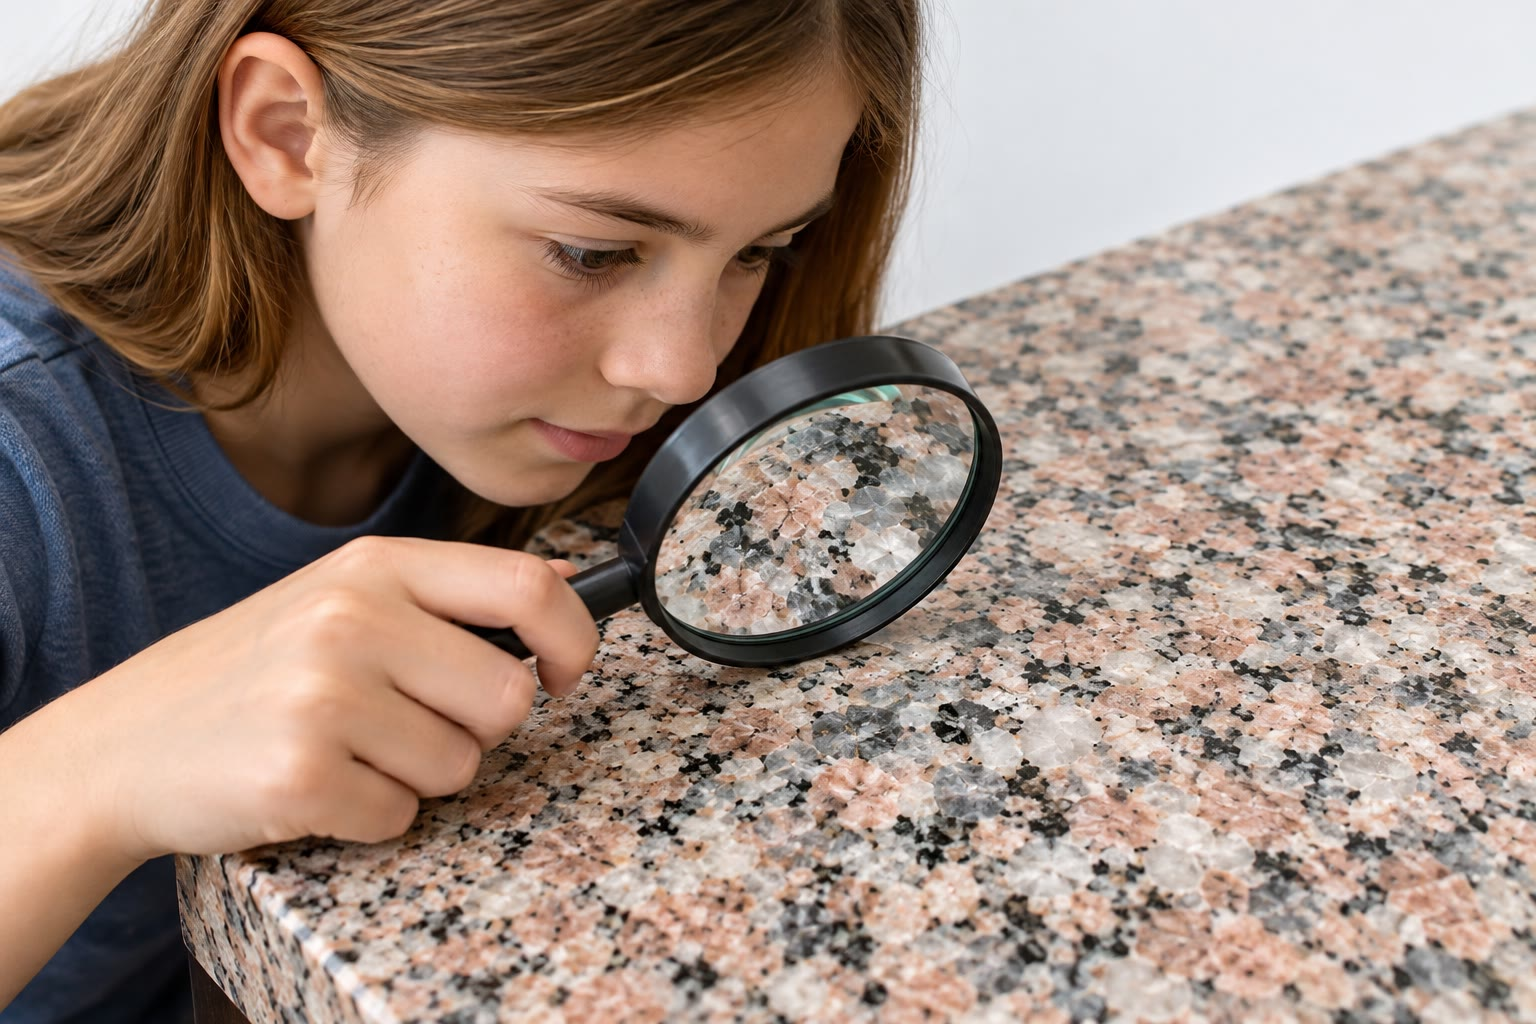
\includegraphics[width=0.6\linewidth]{images/book1/ai/g6-hand-lens-worktop.jpg}

{\small Uma bancada de pedra pintalgada vista através de uma lupa.
(Ilustração feita por IA.)}
\end{omfigure}

\begin{recall}
As \omterm{def:g3:stones-pebbles-sand:rock}{rochas} são o material duro da crosta da Terra: elas podem ser quebradas
em pedras, roladas pelos \omterm{def:g1:landscapes-around-us:water}{rios} até virarem \omterm{def:g3:stones-pebbles-sand:pebble}{seixos} e moídas até virarem
\omterm{def:g3:stones-pebbles-sand:sand}{areia} (\cref{ch:g3:stones-pebbles-sand}). A água, o gelo e o vento
desgastam as \omterm{def:g3:stones-pebbles-sand:rock}{rochas} (\omterm{def:g5:water-shapes-the-land:weathering}{intemperismo}), levam os pedaços embora (\omterm{def:g5:water-shapes-the-land:erosion}{erosão}) e os
deixam mais adiante (\omterm{def:g5:water-shapes-the-land:deposition}{deposição}) (\cref{ch:g5:water-shapes-the-land}). Num
\omterm{def:g4:volcanoes-earthquakes-first-look:volcano}{vulcão}, a \omterm{def:g3:stones-pebbles-sand:rock}{rocha} derretida sai como \omterm{def:g4:volcanoes-earthquakes-first-look:eruption}{lava}
(\cref{ch:g4:volcanoes-earthquakes-first-look}).
\end{recall}

\section{Uma rocha é feita de minerais}

As pintinhas da bancada são \omterm{def:g6:rocks-and-minerals:mineral}{minerais}, e a pedra é um granito.

\begin{definition}[Mineral]\label{def:g6:rocks-and-minerals:mineral}
Um \emph{mineral}\index{mineral} é uma substância sólida natural, que não é
fabricada pelos seres vivos, sempre com a mesma composição e com os seus
átomos arrumados de forma regular. Uma \emph{\omterm{def:g3:stones-pebbles-sand:rock}{rocha}} é feita de um só
mineral ou, mais vezes, de vários minerais grudados uns nos outros.
% ledger: usgs:mineral-rock
\end{definition}

O granito é feito sobretudo de três \omterm{def:g6:rocks-and-minerals:mineral}{minerais}: o \emph{feldspato} (rosado
ou branco), o \emph{quartzo} (cinza e vítreo) e a \emph{mica} (preta ou
prateada, em lâminas finas e brilhantes). Outras \omterm{def:g3:stones-pebbles-sand:rock}{rochas} são feitas de um
só \omterm{def:g6:rocks-and-minerals:mineral}{mineral}: o calcário, por exemplo, é feito quase só de calcita.
% ledger: nps:granite-minerals, usgs:mineral-rock

\begin{omfigure}
\begin{minipage}[c]{0.5\linewidth}\centering
\begin{tikzpicture}
  \begin{axis}[axis equal image, hide axis, width=\linewidth,
      xmin=0, xmax=6, ymin=0, ymax=4]
    \addplot[fill=orange!35!pink, draw=black!55, line width=0.4pt]
      table {figdata/out/grade-6-granite_mosaic-feldspar.dat};
    \addplot[fill=black!12, draw=black!55, line width=0.4pt]
      table {figdata/out/grade-6-granite_mosaic-quartz.dat};
    \addplot[fill=black!85, draw=black!55, line width=0.4pt]
      table {figdata/out/grade-6-granite_mosaic-mica.dat};
  \end{axis}
\end{tikzpicture}

{\small \tikz\fill[orange!35!pink, draw=black!55] (0,0) rectangle (0.25,0.18); feldspato\quad
\tikz\fill[black!12, draw=black!55] (0,0) rectangle (0.25,0.18); quartzo\quad
\tikz\fill[black!85] (0,0) rectangle (0.25,0.18); mica}
\end{minipage}\hfill
\begin{minipage}[c]{0.46\linewidth}\centering
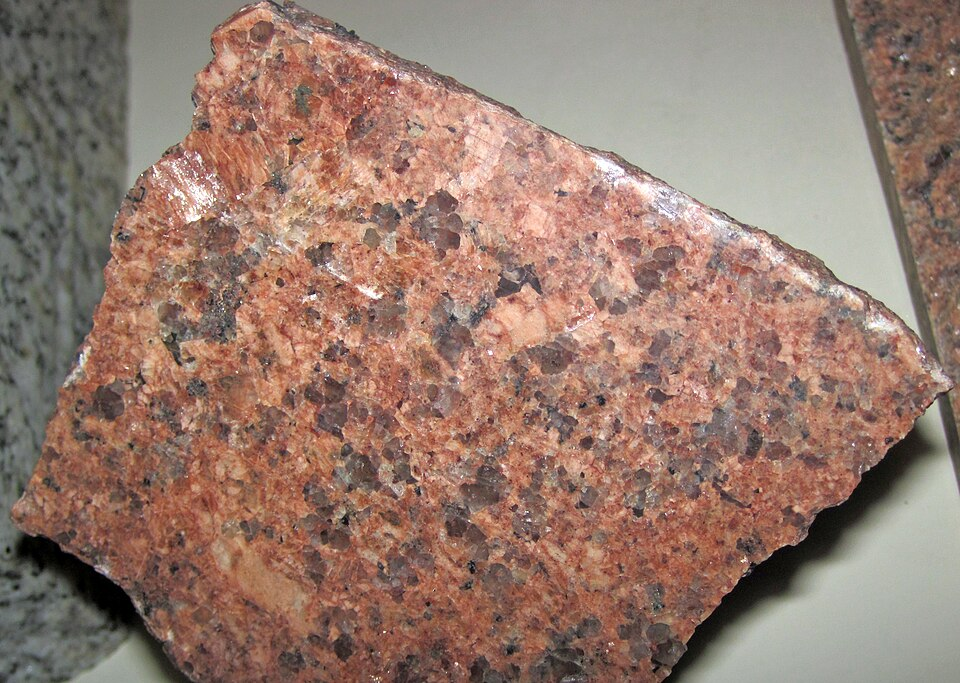
\includegraphics[width=\linewidth]{images/book1/g6-granite.jpg}
\end{minipage}

\smallskip
{\small À esquerda: o granito desenhado como um mosaico de grãos, cada grão
um \omterm{def:g6:rocks-and-minerals:mineral}{mineral} (uma ampliação, fora de escala). À direita: um granito rosado
de verdade, mais ou menos do tamanho de uma mão. (Foto: James St.~John,
CC BY 2.0, via Wikimedia Commons.)}
% ledger: nps:granite-minerals, commons:jsj-rocks (figdata/grade-6/granite_mosaic.py)
\end{omfigure}

\section{Os cristais}

Com a lupa, muitos grãos de \omterm{def:g6:rocks-and-minerals:mineral}{mineral} mostram faces planas e brilhantes e
arestas retas. Onde um \omterm{def:g6:rocks-and-minerals:mineral}{mineral} teve espaço para crescer livremente, num
buraco da \omterm{def:g3:stones-pebbles-sand:rock}{rocha}, ele forma um cristal: um sólido de forma regular,
limitado por faces planas. A sua forma vem do arranjo regular dos seus
átomos, estudado nos livros de química. Um cristal de quartzo, por
exemplo, é uma coluna de seis lados que termina em ponta; um cristal de
mica se divide em folhas mais finas que papel.

\begin{omfigure}
\begin{minipage}[c]{0.2\linewidth}\centering
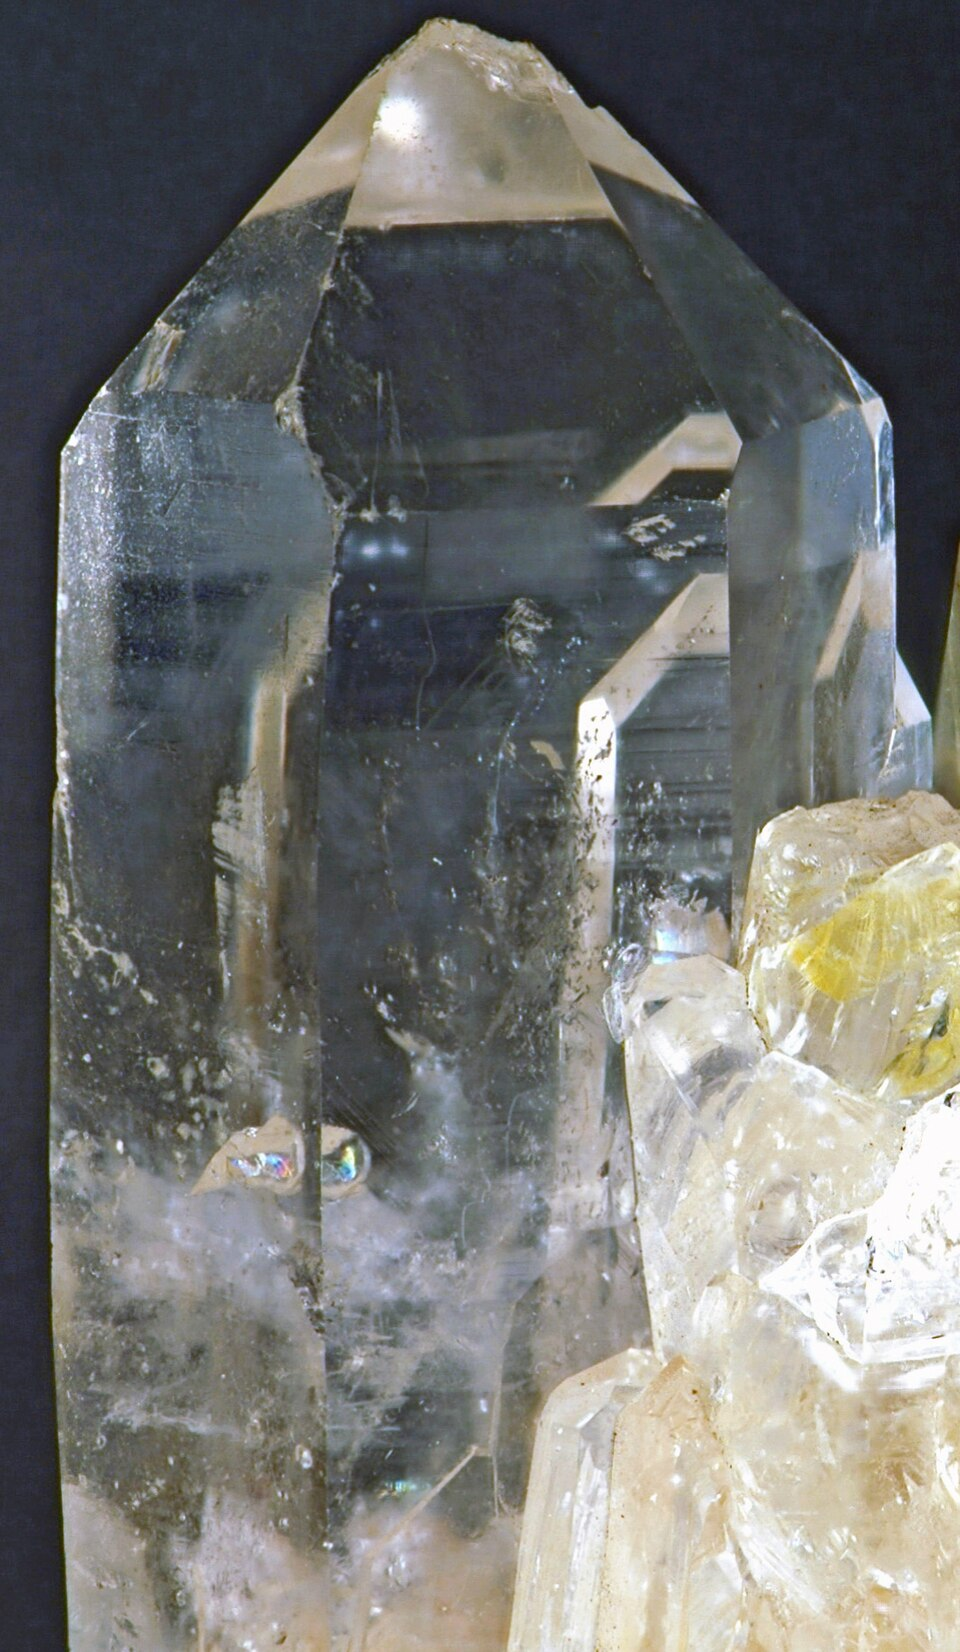
\includegraphics[height=4.2cm]{images/book1/g6-quartz.jpg}
\end{minipage}\hfill
\begin{minipage}[c]{0.44\linewidth}\centering
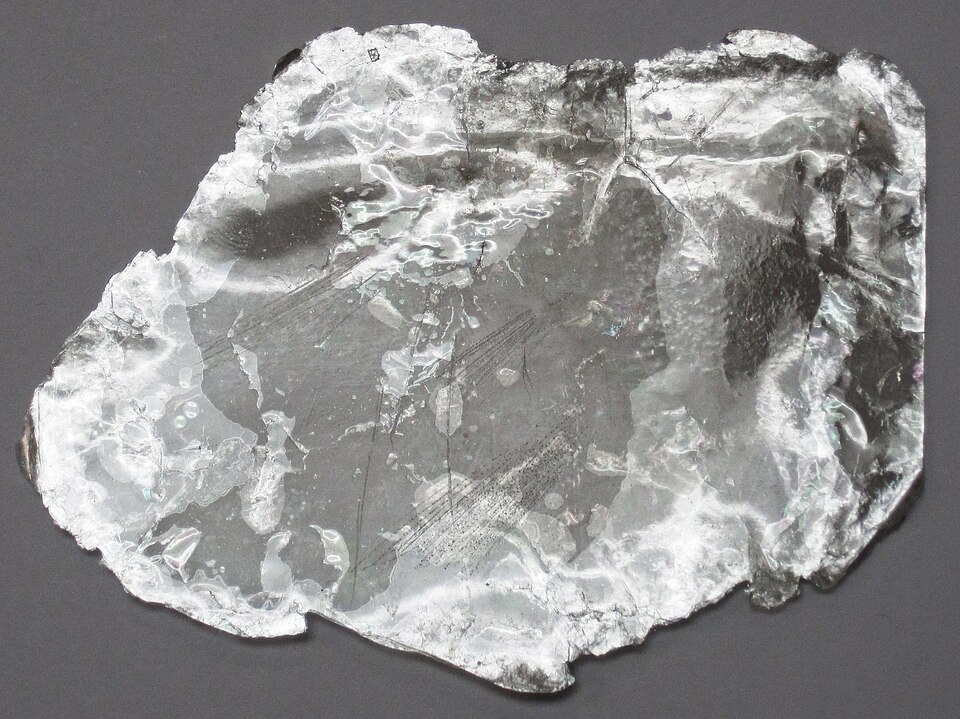
\includegraphics[height=4.2cm]{images/book1/g6-mica.jpg}
\end{minipage}\hfill
\begin{minipage}[c]{0.28\linewidth}
{\small À esquerda: um cristal de quartzo, com as suas faces planas. À
direita: uma folha de mica, um \omterm{def:g6:rocks-and-minerals:mineral}{mineral} que se divide em lâminas muito
finas. (Fotos: James St.~John, CC BY 2.0, via Wikimedia Commons.)}
% ledger: commons:jsj-rocks
\end{minipage}
\end{omfigure}

No granito, os grãos cresceram apertados uns contra os outros, então eles
não têm formas bonitas: eles se encaixam como um quebra-cabeça. O seu
tamanho conta uma história. O granito se forma no fundo da terra, onde a
\omterm{def:g3:stones-pebbles-sand:rock}{rocha} derretida esfria muito devagar: os seus grãos têm tempo de crescer o
bastante para serem vistos a olho nu. A \omterm{def:g3:stones-pebbles-sand:rock}{rocha} derretida que esfria
depressa na superfície, como \omterm{def:g4:volcanoes-earthquakes-first-look:eruption}{lava}, dá \omterm{def:g3:stones-pebbles-sand:rock}{rochas} com grãos pequenos demais
para ver.
% ledger: usgs:mineral-rock

\section{As três famílias de rochas}

Os geólogos classificam as \omterm{def:g3:stones-pebbles-sand:rock}{rochas} em três famílias, não pela sua cor, mas
pela maneira como elas se formaram.

\begin{definition}[As três famílias de rochas]\label{def:g6:rocks-and-minerals:rock-families}
Uma \emph{rocha ígnea}\index{rocha ignea@rocha ígnea} se forma quando uma \omterm{def:g3:stones-pebbles-sand:rock}{rocha} derretida
esfria e fica sólida: o granito no fundo da terra, o basalto a partir da
\omterm{def:g4:volcanoes-earthquakes-first-look:eruption}{lava}. Uma \emph{rocha sedimentar}\index{rocha sedimentar} se forma na
superfície da Terra a partir de grãos de \omterm{def:g3:stones-pebbles-sand:sand}{areia} e de \omterm{def:g3:stones-pebbles-sand:sand}{lama}, ou de conchas de
seres vivos, depositados em camadas e depois endurecidos: o arenito, o
folhelho, o calcário. Uma \emph{rocha metamórfica}\index{rocha metamorfica@rocha metamórfica} é
uma \omterm{def:g3:stones-pebbles-sand:rock}{rocha} que foi transformada, sem derreter, pelo calor e pela pressão no
fundo da terra: o mármore (a partir do calcário), a ardósia (a partir do
folhelho).
% ledger: usgs:mineral-rock, usgs:sedimentary, usgs:metamorphic, geo:marble, geo:slate
\end{definition}

O nome \emph{ígnea} vem da palavra latina que quer dizer fogo. As \omterm{def:g6:rocks-and-minerals:rock-families}{rochas
sedimentares} muitas vezes mostram camadas, uma em cima da outra, como as
páginas de um livro. As \omterm{def:g6:rocks-and-minerals:rock-families}{rochas metamórficas} muitas vezes são espremidas e
dobradas; algumas, como a ardósia, se dividem em placas planas.
% ledger: usgs:mineral-rock, usgs:sedimentary, usgs:metamorphic

Muitas \omterm{def:g6:rocks-and-minerals:rock-families}{rochas sedimentares} são feitas dos grãos que você classificou por
tamanho no \cref{ch:g3:stones-pebbles-sand}: \omterm{def:g3:stones-pebbles-sand:pebble}{seixos} e \omterm{def:g3:stones-pebbles-sand:pebble}{cascalho}, \omterm{def:g3:stones-pebbles-sand:sand}{areia},
\omterm{def:g3:stones-pebbles-sand:sand}{lama}. Depois de enterrados, os grãos perdem a sua água e são grudados uns
nos outros por um cimento natural. O tamanho dos grãos dá o nome à \omterm{def:g3:stones-pebbles-sand:rock}{rocha}.
% ledger: usgs:sedimentary, usgs:wentworth

\begin{omfigure}
\begin{tikzpicture}[
    col/.style={draw=black!60, rounded corners=2pt, minimum width=3.6cm, minimum height=1.9cm},
    lab/.style={font=\scriptsize, align=center}]
  % gravel -> conglomerate
  \node[col, fill=omLithCongl!50] (g) at (0,0) {};
  \foreach \x/\y/\r in {-1.2/0.4/0.32, -0.4/-0.3/0.4, 0.5/0.35/0.3, 1.25/-0.35/0.33, 0.2/-0.55/0.18, -1.3/-0.5/0.22}
    \fill[gray!55, draw=black!60] (\x,\y) circle (\r);
  \node[lab, above=2pt] at (g.north) {\textbf{cascalho}\\ mais de 2~mm};
  \node[lab, below=3pt] (cg) at (g.south) {$\downarrow$ enterrado e cimentado\\ \textbf{conglomerado}};
    % sand -> sandstone
  \pgfmathsetseed{7}

  \node[col, fill=omLithSand!60] (s) at (4.2,0) {};
  \foreach \i in {1,...,70} \fill[brown!60!black] ({4.2+1.65*rand},{0.82*rand}) circle (0.045);
  \node[lab, above=2pt] at (s.north) {\textbf{areia}\\ de 2~mm a $\frac{1}{16}$~mm};
  \node[lab, below=3pt] at (s.south) {$\downarrow$ enterrada e cimentada\\ \textbf{arenito}};
  % mud -> shale
  \node[col, fill=omLithShale!70] (m) at (8.4,0) {};
  \foreach \y in {-0.75,-0.5,...,0.8} \draw[black!35, line width=0.3pt] (6.75,\y) -- (10.05,\y);
  \node[lab, above=2pt] at (m.north) {\textbf{lama} (silte e argila)\\ menos de $\frac{1}{16}$~mm};
  \node[lab, below=3pt] at (m.south) {$\downarrow$ enterrada e prensada\\ \textbf{folhelho}};
\end{tikzpicture}

{\small Três \omterm{def:g6:rocks-and-minerals:rock-families}{rochas sedimentares} que recebem o nome do tamanho dos seus
grãos (grãos muito ampliados; a \omterm{def:g3:stones-pebbles-sand:sand}{areia} mostrada na escala da caixa, o
\omterm{def:g3:stones-pebbles-sand:pebble}{cascalho} maior).}
% ledger: usgs:wentworth, usgs:sedimentary
\end{omfigure}

\begin{inthefield}[Ler as pedras de uma cidade]
As cidades são coleções de \omterm{def:g3:stones-pebbles-sand:rock}{rochas} ao ar livre. Passeie com um adulto perto
de muros antigos, escadas, estátuas, fachadas de igrejas e calçamentos, e
observe de perto, sem riscar nem quebrar nada. Alguns meios-fios e degraus são de granito: procure o seu quartzo vítreo e a sua mica brilhante. Muitos muros e fachadas antigos são de calcário ou de arenito: procure conchas, ou esfregue a ponta do dedo num farelo caído de
arenito para sentir a \omterm{def:g3:stones-pebbles-sand:sand}{areia}. Os telhados podem ser de ardósia, dividida em
placas finas. Anote num caderno onde fica cada pedra, a sua cor, os seus
grãos e a família à qual você acha que ela pertence; uma foto ajuda a
comparar depois com a tabela deste capítulo.
\end{inthefield}

\section{O ciclo das rochas}

As \omterm{def:g3:stones-pebbles-sand:rock}{rochas} não são eternas. Uma \omterm{def:g1:landscapes-around-us:landform}{montanha} de granito sofre \omterm{def:g5:water-shapes-the-land:weathering}{intemperismo}
devagar; os seus grãos são levados pelos \omterm{def:g1:landscapes-around-us:water}{rios} até o \omterm{def:g2:water-on-earth:ocean}{mar} e depositados ali
em camadas; enterradas cada vez mais fundo, as camadas endurecem e viram
arenito. Se o arenito for levado ainda mais fundo, o calor e a pressão o
transformam numa \omterm{def:g6:rocks-and-minerals:rock-families}{rocha metamórfica}; ainda mais fundo, ele pode derreter,
e a \omterm{def:g3:stones-pebbles-sand:rock}{rocha} derretida, ao esfriar, forma uma nova \omterm{def:g6:rocks-and-minerals:rock-families}{rocha ígnea}. Pouco a
pouco, ao longo de milhões de anos, o material das \omterm{def:g3:stones-pebbles-sand:rock}{rochas} dá voltas e
mais voltas.
% ledger: usgs:sedimentary, usgs:metamorphic

\begin{definition}[Ciclo das rochas]\label{def:g6:rocks-and-minerals:rock-cycle}
O \emph{ciclo das rochas}\index{ciclo das rochas} é a viagem sem fim pela
qual as \omterm{def:g3:stones-pebbles-sand:rock}{rochas} de cada família vão sendo transformadas, devagar, em \omterm{def:g3:stones-pebbles-sand:rock}{rochas}
das outras famílias: pelo \omterm{def:g5:water-shapes-the-land:weathering}{intemperismo} e pela \omterm{def:g5:water-shapes-the-land:erosion}{erosão} na superfície, pelo
soterramento e pelo endurecimento, pelo calor e pela pressão, pela fusão e
pelo resfriamento.
\end{definition}

\begin{omfigure}
\begin{tikzpicture}[
    fam/.style={draw, rounded corners=4pt, thick, align=center, minimum width=3.2cm,
                minimum height=1.0cm, font=\small\bfseries},
    stage/.style={draw, dashed, rounded corners=4pt, align=center, minimum width=3.0cm,
                  minimum height=0.9cm, font=\small},
    arr/.style={-{Stealth[length=2.6mm]}, thick},
    lab/.style={font=\scriptsize, align=center, fill=white, inner sep=1.5pt}]
  \node[fam, fill=omLithGranite!60] (ign) at (0,3.6) {rochas ígneas\\[-1pt]{\normalfont\scriptsize granito, basalto}};
  \node[stage, fill=orange!15] (grains) at (6.6,3.6) {grãos de areia\\e de lama};
  \node[fam, fill=omLithSand!70] (sed) at (6.6,0) {rochas sedimentares\\[-1pt]{\normalfont\scriptsize arenito, folhelho, calcário}};
  \node[fam, fill=omLithSchist!60] (met) at (0,0) {rochas metamórficas\\[-1pt]{\normalfont\scriptsize mármore, ardósia}};
  \node[stage, fill=red!12] (melt) at (-4.2,1.8) {rocha derretida\\no fundo da terra};
  \draw[arr] (ign) -- node[lab, above] {intemperismo\\e erosão} (grains);
  \draw[arr] (grains) -- node[lab, right] {depositados em camadas,\\enterrados, endurecidos} (sed);
  \draw[arr] (sed) -- node[lab, below=2pt] {calor e pressão,\\no fundo da terra} (met);
  \draw[arr] (met) -- node[lab, below left] {fusão} (melt);
  \draw[arr] (melt) -- node[lab, above left] {resfriamento} (ign);
  \draw[arr, black!55] (met.north east) to[bend left=12] node[lab, pos=0.45, left=4pt, text=black!60] {intemperismo} ([xshift=-6pt]grains.south west);
  \draw[arr, black!55] (sed.north west) to[bend left=10] (grains.south west);
\end{tikzpicture}

{\small O \omterm{def:g6:rocks-and-minerals:rock-cycle}{ciclo das rochas}. Cada seta leva de milhares a milhões de anos.
Qualquer \omterm{def:g3:stones-pebbles-sand:rock}{rocha} que sobe até a superfície pode sofrer \omterm{def:g5:water-shapes-the-land:weathering}{intemperismo} (setas
cinzentas).}
% ledger: usgs:sedimentary, usgs:metamorphic, usgs:mineral-rock
\end{omfigure}

\section{Reconhecer as rochas comuns}

Aqui estão sete \omterm{def:g3:stones-pebbles-sand:rock}{rochas} que encontramos muitas vezes em construções,
calçadas e \omterm{def:g1:landscapes-around-us:landscape}{paisagens}.

\begin{omfigure}
\newcommand{\gsixrock}[2]{\begin{minipage}[t]{0.235\linewidth}\centering
  \includegraphics[width=\linewidth, height=0.72\linewidth, keepaspectratio=false]{images/book1/#1}\\[1pt]
  {\footnotesize #2}\end{minipage}}
\gsixrock{g6-granite.jpg}{granito}\hfill
\gsixrock{g6-basalt.jpg}{basalto}\hfill
\gsixrock{g6-sandstone.jpg}{arenito}\hfill
\gsixrock{g6-limestone.jpg}{calcário (com conchas)}\par\medskip
\gsixrock{g6-shale.jpg}{folhelho}\hspace{0.02\linewidth}%
\gsixrock{g6-marble.jpg}{mármore}\hspace{0.02\linewidth}%
\gsixrock{g6-slate-roof.jpg}{ardósia, num telhado}

\medskip
{\small Sete \omterm{def:g3:stones-pebbles-sand:rock}{rochas} comuns. (Fotos: James St.~John, CC BY 2.0; telhado:
Øyvind Holmstad, CC0; via Wikimedia Commons.)}
% ledger: commons:jsj-rocks, commons:roof-slates
\end{omfigure}

\begin{center}
\small
\begin{tabular}{>{\raggedright\arraybackslash}p{0.13\linewidth}>{\raggedright\arraybackslash}p{0.15\linewidth}>{\raggedright\arraybackslash}p{0.6\linewidth}}
\hline
\omterm{def:g3:stones-pebbles-sand:rock}{rocha} & família & o que procurar\\
\hline
granito & ígnea & grãos grandes de várias cores: feldspato rosado ou branco, quartzo cinza e vítreo, mica preta e brilhante\\
basalto & ígnea & cinza-escuro a preto, grãos pequenos demais para ver, muitas vezes com buraquinhos redondos deixados por bolhas de gás\\
arenito & sedimentar & grãos de \omterm{def:g3:stones-pebbles-sand:sand}{areia} que dá para sentir, áspero como lixa\\
calcário & sedimentar & claro, muitas vezes com conchas; faz efervescência com uma gota de ácido diluído\\
folhelho & sedimentar & muito fino e mole, feito de \omterm{def:g3:stones-pebbles-sand:sand}{lama} endurecida (argila); em camadas finas\\
mármore & metamórfica & branco ou colorido, feito de cristais brilhantes que cintilam como açúcar; faz efervescência com ácido\\
ardósia & metamórfica & cinza, muito fina, se divide em placas finas, duras e planas\\
\hline
\end{tabular}
% ledger: nps:granite-minerals, geo:basalt, usgs:sedimentary, geo:limestone, geo:marble, geo:slate
\end{center}

\begin{safety}
O teste do ácido só é feito por um adulto, com óculos de proteção e luvas,
usando um ácido muito diluído. Nunca prove uma \omterm{def:g3:stones-pebbles-sand:rock}{rocha} ou um pó, e nunca
quebre \omterm{def:g3:stones-pebbles-sand:rock}{rochas} com uma ferramenta: olhar através de uma lupa já diz muita
coisa.
% ledger: geo:limestone
\end{safety}

Uma chave é uma lista de perguntas, cada uma com duas respostas, que leva
passo a passo ao nome de uma \omterm{def:g3:stones-pebbles-sand:rock}{rocha}.

\begin{omfigure}
\begin{tikzpicture}[
    q/.style={draw, rounded corners=3pt, fill=omRecall!10, align=center, text width=3.7cm,
              font=\scriptsize, inner sep=3pt},
    r/.style={draw, rounded corners=3pt, thick, fill=omLithSand!40, font=\scriptsize\bfseries,
              align=center, minimum width=1.7cm, inner sep=3pt},
    arr/.style={-{Stealth[length=2mm]}, thick}, yn/.style={font=\scriptsize\itshape, fill=white, inner sep=1pt}]
  \node[q] (q1) at (0,0) {Faz efervescência com uma gota de ácido diluído?};
  \node[q] (q2) at (-3.4,-1.6) {Dá para ver conchas, ou ela parece fosca e fina?};
  \node[r] (lime) at (-4.8,-3.4) {calcário};
  \node[r, align=center] (marb) at (-2.0,-3.4) {mármore\\[-1pt]{\normalfont\tiny cristais brilhantes}};
  \node[q] (q3) at (3.2,-1.6) {Dá para ver grãos de várias cores, rosados, cinza, pretos?};
  \node[r] (gran) at (6.9,-1.6) {granito};
  \node[q] (q4) at (3.2,-3.2) {Escura, com grãos pequenos demais para ver, buraquinhos redondos?};
  \node[r] (bas) at (6.9,-3.2) {basalto};
  \node[q] (q5) at (3.2,-4.8) {Áspera como lixa, feita de grãos de areia?};
  \node[r] (sand) at (6.9,-4.8) {arenito};
  \node[q] (q6) at (3.2,-6.4) {Dura, se dividindo em placas finas e planas?};
  \node[r] (slat) at (6.9,-6.4) {ardósia};
  \node[r] (shal) at (3.2,-7.8) {folhelho};
  \draw[arr] (q1) -| node[yn, pos=0.25] {sim} (q2);
  \draw[arr] (q1) -| node[yn, pos=0.25] {não} (q3);
  \draw[arr] (q2.south-|lime) -- node[yn, right] {sim} (lime);
  \draw[arr] (q2.south-|marb) -- node[yn, right] {não} (marb);
  \foreach \a/\b in {q3/gran, q4/bas, q5/sand, q6/slat}{\draw[arr] (\a) -- node[yn, above] {sim} (\b);}
  \foreach \a/\b in {q3/q4, q4/q5, q5/q6, q6/shal}{\draw[arr] (\a) -- node[yn, right] {não} (\b);}
\end{tikzpicture}

{\small Uma chave para as sete \omterm{def:g3:stones-pebbles-sand:rock}{rochas} da tabela. Comece no alto e responda
a cada pergunta com sim ou não.}
% ledger: geo:limestone, geo:marble, nps:granite-minerals, geo:basalt, usgs:sedimentary, geo:slate
\end{omfigure}

\paragraph{A dureza.} Mais uma pista ajuda a reconhecer um \omterm{def:g6:rocks-and-minerals:mineral}{mineral}: a
facilidade com que ele pode ser riscado.

\begin{definition}[Dureza e escala de Mohs]\label{def:g6:rocks-and-minerals:hardness}
A \emph{dureza}\index{dureza} de um \omterm{def:g6:rocks-and-minerals:mineral}{mineral} é quanto ele resiste a ser
riscado: um \omterm{def:g6:rocks-and-minerals:mineral}{mineral} risca todos os mais moles e é riscado por todos os mais
duros. A \emph{escala de Mohs}\index{escala de Mohs} classifica a dureza de 1 a
10 com dez \omterm{def:g6:rocks-and-minerals:mineral}{minerais} de referência, do talco (1), o mais mole, ao diamante
(10), o mais duro.
% ledger: nps:mohs-ladder, nps:mohs-testers
\end{definition}

\begin{omfigure}
\begin{tikzpicture}[x=1cm, y=0.62cm]
  \draw[thick, black!60] (0,0.5) -- (0,10.5);
  \foreach \n/\m in {1/talco, 2/gipsita, 3/calcita, 4/fluorita, 5/apatita,
                     6/feldspato (ortoclásio), 7/quartzo, 8/topázio, 9/coríndon, 10/diamante}{
    \fill[omRecall!25, draw=black!50] (-0.32,\n-0.32) rectangle (0.32,\n+0.32);
    \node[font=\scriptsize\bfseries] at (0,\n) {\n};
    \node[font=\scriptsize, anchor=east] at (-0.5,\n) {\m};}
  \foreach \v/\t in {2.5/unha, 3.5/moeda de cobre, 5.5/vidro, 6.5/prego de aço}{
    \draw[red!70!black, thick] (0.4,\v) -- (1.0,\v);
    \node[font=\scriptsize, red!70!black, anchor=west] at (1.05,\v) {\t\ (cerca de \v)};}
  \node[font=\scriptsize\itshape, anchor=south] at (0,10.6) {mais duro};
  \node[font=\scriptsize\itshape, anchor=north] at (0,0.4) {mais mole};
  \node[font=\scriptsize, align=left, anchor=west, text width=6.2cm] at (4.3,5.5)
    {Uma unha risca o talco e a gipsita, mas não a calcita. Uma moeda de
     cobre risca a calcita. O quartzo risca o vidro e o aço; nenhum dos quatro testadores risca o quartzo. A mica, entre 2 e 3, mal pode ser riscada por uma
     unha.};
\end{tikzpicture}

{\small A \omterm{def:g6:rocks-and-minerals:hardness}{escala de Mohs} (à esquerda: os dez \omterm{def:g6:rocks-and-minerals:mineral}{minerais} de referência) e
quatro testadores do dia a dia (à direita, em vermelho).}
% ledger: nps:mohs-ladder, nps:mohs-testers, geo:mica-hardness
\end{omfigure}

\begin{method}[O teste do risco]\label{met:g6:rocks-and-minerals:scratch}
\begin{enumerate}
  \item Tente riscar o \omterm{def:g6:rocks-and-minerals:mineral}{mineral} com a unha, depois com uma moeda de cobre.
        (O vidro e o aço só são usados por um adulto.)
  \item Esfregue a marca com o dedo: um risco de verdade fica, e um rastro
        de pó deixado pelo testador sai.
  \item A \omterm{def:g6:rocks-and-minerals:hardness}{dureza} fica entre a do testador mais duro que não o risca e a do
        testador mais mole que o risca.
\end{enumerate}
\end{method}

\begin{example}[Quartzo ou calcita?]\label{ex:g6:rocks-and-minerals:quartz-calcite}
Dois \omterm{def:g6:rocks-and-minerals:mineral}{minerais} brancos se parecem. O primeiro é riscado por uma moeda de
cobre: a sua \omterm{def:g6:rocks-and-minerals:hardness}{dureza} é menor que 3.5; é a calcita (3). O segundo não é
riscado por um prego de aço e risca o vidro: a sua \omterm{def:g6:rocks-and-minerals:hardness}{dureza} é maior que
6.5; entre os \omterm{def:g6:rocks-and-minerals:mineral}{minerais} de referência, é o quartzo (7).
% ledger: nps:mohs-ladder, nps:mohs-testers
\end{example}

\section{Exercícios}

\begin{exercise}[$\star$]\label{exo:g6:rocks-and-minerals:1}
A que família pertence cada \omterm{def:g3:stones-pebbles-sand:rock}{rocha}: granito, arenito, mármore, basalto,
calcário, ardósia?
\end{exercise}

\begin{exercise}[$\star$]\label{exo:g6:rocks-and-minerals:2}
O quartzo é um \omterm{def:g6:rocks-and-minerals:mineral}{mineral} ou uma \omterm{def:g3:stones-pebbles-sand:rock}{rocha}? E o granito? Explique a diferença em
uma frase.
\end{exercise}

\begin{exercise}[$\star$]\label{exo:g6:rocks-and-minerals:3}
Coloque estes \omterm{def:g6:rocks-and-minerals:mineral}{minerais} em ordem, do mais mole ao mais duro: quartzo,
talco, diamante, calcita. Qual deles consegue riscar todos os outros?
\end{exercise}

\begin{exercise}[$\star$]\label{exo:g6:rocks-and-minerals:4}
Copie e complete com as palavras \emph{resfriamento}, \emph{calor e
pressão}, \emph{\omterm{def:g5:water-shapes-the-land:weathering}{intemperismo}}: ``A \omterm{def:g3:stones-pebbles-sand:rock}{rocha} derretida vira uma \omterm{def:g6:rocks-and-minerals:rock-families}{rocha ígnea} por
\ldots{} Um calcário vira um mármore por \ldots{} Um granito se transforma
em grãos de \omterm{def:g3:stones-pebbles-sand:sand}{areia} por \ldots''
\end{exercise}

\begin{exercise}[$\star\star$]\label{exo:g6:rocks-and-minerals:5}
Use a chave. (a) Uma \omterm{def:g3:stones-pebbles-sand:rock}{rocha} não faz efervescência com ácido; ela é escura,
com grãos pequenos demais para ver e buraquinhos redondos. (b) Uma \omterm{def:g3:stones-pebbles-sand:rock}{rocha}
faz efervescência com ácido e é feita de cristais brilhantes que cintilam
como açúcar. (c) Uma \omterm{def:g3:stones-pebbles-sand:rock}{rocha} não faz efervescência; ela é áspera como lixa.
Dê o nome de cada \omterm{def:g3:stones-pebbles-sand:rock}{rocha}.
\end{exercise}

\begin{exercise}[$\star\star$]\label{exo:g6:rocks-and-minerals:6}
Um \omterm{def:g6:rocks-and-minerals:mineral}{mineral} é riscado por uma moeda de cobre, mas não pela unha. Entre que
dois valores de \omterm{def:g6:rocks-and-minerals:hardness}{dureza} ele fica? Que \omterm{def:g6:rocks-and-minerals:mineral}{mineral} de referência da \omterm{def:g6:rocks-and-minerals:hardness}{escala de
Mohs} ele poderia ser?
\end{exercise}

\begin{exercise}[$\star\star$]\label{exo:g6:rocks-and-minerals:7}
% exercise data: figdata/grade-6/granite_mosaic.py (33 / 21 / 6 grains)
No desenho do granito deste capítulo, há 60 grãos: 33 de feldspato, 21 de
quartzo e 6 de mica. Que porcentagem dos grãos é de quartzo? E de
feldspato? E de mica? Verifique que as três porcentagens somam
100~\%.
\end{exercise}

\begin{exercise}[$\star\star$]\label{exo:g6:rocks-and-minerals:8}
O granito e o basalto são as duas \omterm{def:g6:rocks-and-minerals:rock-families}{rochas ígneas}. Por que conseguimos ver
os grãos do granito a olho nu, mas não os do basalto?
\end{exercise}

\begin{exercise}[$\star\star$]\label{exo:g6:rocks-and-minerals:9}
O mármore é formado a partir do calcário. (a) A que família pertence cada
um? (b) O que aconteceu com o calcário para transformá-lo em mármore?
(c) Por que os dois fazem efervescência com ácido?
\end{exercise}

\begin{exercise}[$\star\star$]\label{exo:g6:rocks-and-minerals:10}
Usando a \omterm{def:g6:rocks-and-minerals:hardness}{escala de Mohs}: (a) o quartzo consegue riscar uma garrafa de
vidro? (b) E a fluorita? (c) Um prego de aço consegue riscar o feldspato?
\end{exercise}

\begin{exercise}[$\star\star\star$]\label{exo:g6:rocks-and-minerals:11}
Conte a viagem de um grão de quartzo, em cinco etapas, de uma \omterm{def:g1:landscapes-around-us:landform}{montanha} de
granito até uma \omterm{def:g6:rocks-and-minerals:rock-families}{rocha metamórfica}. Dê o nome do processo em cada etapa, e a
família da \omterm{def:g3:stones-pebbles-sand:rock}{rocha} no começo e no fim.
\end{exercise}

\begin{exercise}[$\star\star\star$]\label{exo:g6:rocks-and-minerals:12}
Um \omterm{def:g6:rocks-and-minerals:mineral}{mineral} cinza e vítreo não é riscado por um prego de aço, risca o vidro
e é riscado pelo topázio. (a) Qual é a sua \omterm{def:g6:rocks-and-minerals:hardness}{dureza} na \omterm{def:g6:rocks-and-minerals:hardness}{escala de Mohs}? Dê o
seu nome. (b) Os grãos de \omterm{def:g3:stones-pebbles-sand:sand}{areia} são rolados durante anos pelas ondas e
pelos \omterm{def:g1:landscapes-around-us:water}{rios}. Usando a sua \omterm{def:g6:rocks-and-minerals:hardness}{dureza}, explique por que os grãos desse \omterm{def:g6:rocks-and-minerals:mineral}{mineral}
duram muito mais que os grãos de calcita ou de mica.
\end{exercise}

\section{Problema: As pedras da praça da cidade}

\begin{problem}[{Problema de fim de semana --- as rochas de uma praça, o
mineral mais duro entre elas e quantas famílias de rochas estão presentes}]
\label{pb:g6:rocks-and-minerals:1}
% ledger: nps:granite-minerals, geo:limestone, geo:slate, geo:marble, nps:mohs-ladder, nps:mohs-testers, geo:mica-hardness
Num passeio da escola, a turma observa as pedras da praça antiga da cidade
(só observa: ninguém quebra nem risca os monumentos). A professora trouxe
do depósito de um canteiro pedaços soltos das mesmas pedras para os testes
de \omterm{def:g6:rocks-and-minerals:hardness}{dureza}.

\smallskip
\noindent\textbf{O chafariz}: a sua bacia mostra grãos grandes, rosados,
        brancos, cinzentos e vítreos, e pretos e brilhantes.
\textbf{O calçamento}: lajes claras nas quais se veem pequenas conchas
        fósseis; uma gota de ácido diluído, posta pela professora num
        pedaço solto, faz efervescência.
\textbf{O telhado da prefeitura}: placas finas, planas e cinzentas de uma
        pedra de grãos muito finos.
\textbf{A estátua}: uma pedra branca feita de cristais brilhantes que
        cintilam como açúcar; ela também faz efervescência.

\medskip
\noindent\textbf{Parte I --- O chafariz, o calçamento, o telhado.}
\begin{enumerate}
  \item Dê o nome da \omterm{def:g3:stones-pebbles-sand:rock}{rocha} do chafariz e a sua família. Dê o nome dos seus
        três \omterm{def:g6:rocks-and-minerals:mineral}{minerais}.
  \item Dê o nome da \omterm{def:g3:stones-pebbles-sand:rock}{rocha} do calçamento e a sua família. O que eram as
        conchas antes de estarem na pedra?
  \item Dê o nome da \omterm{def:g3:stones-pebbles-sand:rock}{rocha} do telhado e a sua família. A partir de que
        \omterm{def:g3:stones-pebbles-sand:rock}{rocha} ela se formou?
  \item Dê o nome da \omterm{def:g3:stones-pebbles-sand:rock}{rocha} da estátua e a sua família. A partir de que
        \omterm{def:g3:stones-pebbles-sand:rock}{rocha} ela se formou?
\end{enumerate}

\medskip
\noindent\textbf{Parte II --- Um teste de dureza.}
\begin{enumerate}[resume]
  \item A professora tenta riscar um grão cinza e vítreo do chafariz com um
        prego de aço: nenhum risco. O grão risca o vidro. Que \omterm{def:g6:rocks-and-minerals:mineral}{mineral} é
        esse, e qual é a sua \omterm{def:g6:rocks-and-minerals:hardness}{dureza}?
  \item Os grãos rosados são riscados pelo prego de aço, mas não pelo
        vidro. Entre que dois valores fica a sua \omterm{def:g6:rocks-and-minerals:hardness}{dureza}? Que \omterm{def:g6:rocks-and-minerals:mineral}{mineral} da
        \omterm{def:g6:rocks-and-minerals:hardness}{escala de Mohs} é esse?
  \item As lâminas pretas mal podem ser riscadas pela unha. Que \omterm{def:g6:rocks-and-minerals:mineral}{mineral} é
        esse?
  \item Uma moeda de cobre consegue riscar o calçamento? Explique com a
        \omterm{def:g6:rocks-and-minerals:hardness}{dureza} da calcita.
\end{enumerate}

\medskip
\noindent\textbf{Parte III --- O ciclo das rochas.}
\begin{enumerate}[resume]
  \item Depois de séculos de \omterm{def:g4:clouds-rain-snow:precipitation}{chuva}, a estátua perdeu os seus detalhes
        finos. Que processo do \omterm{def:g6:rocks-and-minerals:rock-cycle}{ciclo das rochas} está agindo?
  \item O granito do chafariz veio de uma \omterm{def:g1:landscapes-around-us:landform}{montanha}. Ao longo de milhões de
        anos, o que poderia acontecer com os grãos de quartzo dessa
        \omterm{def:g1:landscapes-around-us:landform}{montanha}, e em que \omterm{def:g3:stones-pebbles-sand:rock}{rocha} eles poderiam terminar?
  \item Quantas das três famílias de \omterm{def:g3:stones-pebbles-sand:rock}{rochas} estão presentes na praça? Dê o
        nome da \omterm{def:g3:stones-pebbles-sand:rock}{rocha} ou das \omterm{def:g3:stones-pebbles-sand:rock}{rochas} de cada uma.
  \item Qual é a \omterm{def:g6:rocks-and-minerals:hardness}{dureza} de Mohs do \omterm{def:g6:rocks-and-minerals:mineral}{mineral} mais duro encontrado nas pedras
        da praça?
\end{enumerate}
\end{problem}
